\documentclass[journal,a4paper,11pt]{IEEEtran}

\usepackage[utf8]{inputenc}
\usepackage[portuguese]{babel}
\usepackage[version=3]{mhchem}
\usepackage{listings}
\usepackage{graphicx}
\usepackage{url}     
\usepackage{amsmath,bm} 
\usepackage{hyperref}
\usepackage[affil-it]{authblk} 
\usepackage{cite}
\usepackage{babel}
\usepackage{tikz}
\usetikzlibrary{babel}
\usepackage{siunitx}


\begin{document}


\begin{center}
\vspace{0.2cm}
	
	\textbf{Teoria da informação e estatística computacional no processamento e análise de sinais - Implementações otimizadas em \texttt R}\\ 
    
	Eduarda T.\ C.\ Chagas$^{1}$, Alejandro C.\ Frery$^{2}$\\
     $^{1}$Estudante de IC de Ciência da Computação, Ufal
     $^{2}$Laboratório de Computação Científica e Análise Numérica, Ufal
    
\end{center}
\section*{\textbf{Resumo}}

	Este trabalho relata o processo de desenvolvimento de uma plataforma de análise dos descritores causais de uma série temporal oriundos da Teoria da Informação.
 	A plataforma visa facilitar a análise dessas séries nos mais variados ramos da ciência. 
 	O sistema foi implementado na linguagem de programação \texttt R, que além de fornecer ferramentas gráficas, também possui uma grande precisão numérica. 
 	Ambas as características de extrema importância ao longo deste trabalho.
 Após comentar brevemente a respeito de conceitos da Teoria da Informação necessários no processo de análise e modelagem de uma série temporal, expomos os resultados alcançados no decorrer do projeto e sugestões para futuros trabalhos.\\

\textbf{Palavras-chave:} Séries temporais; teoria da informação; linguagem \texttt R.\\

\textbf{Apoio financeiro:} CNPq (Conselho Nacional de Desenvolvimento Científico e Tecnológico).\\

\textbf{Trabalho selecionado para a JNIC pela instituição:} UFAL.

\section*{\textbf{Introdução}}

	Séries temporais são conjunto de dados obtidos a partir de um processo observacional ao longo de um determinado período de tempo, não necessariamente dividido em espaços iguais, sendo caracterizadas pela dependência serial existente entre as observações.
 
 A análise de séries temporais tem vasta aplicabilidade na análise de dados bancários e de finanças, na caracterização de redes de computadores e veiculares, na descrição de sinais biológicos, além de inúmeras outras áreas.
 
 A hipótese subjacente a toda análise de séries temporais é que os dados observados são o resultado da operação de um sistema causal sujeito a ruído observacional.
 Esse sistema, ou dinâmica, é responsável pela criação de padrões através de cuja observação deseja-se inferir a respeito da dinâmica.
 
 A análise de séries temporais é um ramo clássico da Estatística~\cite{BrockwellDavis91} que se divide, tipicamente, na análise no domínio do tempo e no domínio da frequência.
 Ambas abordagens empregam diretamente os valores observados e, portanto, são suscetíveis ao efeito danoso de diversos tipos de contaminação.
 Uma forma de tornar as análises mais imunes a contaminação é através de técnicas robustas~\cite{BustosFraiman1984}.
 Outra, mais moderna, é pelo uso de métodos não-paramétricos.
 
 Há diversas ferramentas que auxiliam na análise clássica de séries temporais; na data de redação deste trabalho havia \num{234} bibliotecas para essa finalidade (ver \url{https://cran.r-project.org/web/views/TimeSeries.html}).
 	Para essa mesma plataforma, apenas três delas bibliotecas trabalham exclusivamente com técnicas não paramétricas.
    
O projeto aqui relatado tomou como ponto de partida a identificação das necessidades dos pesquisadores que trabalham com estas ferramentas: uma ferramenta gráfica amigável e funcionalidades rápidas, eficientes e numericamente confiáveis.
 Outro requisito foi o da portabilidade para diversos sistemas operacionais e arquiteturas de hardware, e o uso de ferramentas FLOSS (\textit{Free/Libre Open Source Software}).
 
 Apresentamos, assim, o desenvolvimento de uma ferramenta portável, rápida e de boa qualidade numérica que possibilita análises interativas e exploratórias dos dados de uma série temporal através de técnicas provenientes da Teoria da Informação.
 Com ela, o usuário dispõe de uma conjunto técnicas de análise presentes na literatura para processar e examinar seus dados de modo eficiente e com um mínimo período de aprendizado.
 A ferramenta é extensível.
    
\section*{\textbf{Metodologia}}

A primeira parte do projeto consistiu da apropriação do referencial teórico.
 Seja a série temporal $\bm x = (x_1, x_2, \dots, x_n)$.
 Ao invés de analisarmos os valores, transformaremos grupos de $N$ valores (não necessariamente adjacentes) e padrões ordinais, e analisaremos a sua distribuição de frequência.
 Por exemplo e sem perda de generalidade, com $N=3$ e para qualquer $i$ viável,
 se $x_i<x_{i+1}<x_{i+2}$ assignaremos a esta tripla o padrão $\pi_0$;
 caso $x_i>x_{i+1}>x_{i+2}$ o padrão será $\pi_1$ e assim por diante.
 Com isso, há $N!$ possíveis padrões.
 Forma-se, então, um histograma e, a partir dele, extraem-se quantificadores como, por exemplo, entropia, distância estocástica a uma distribuição de equilíbrio, e complexidade estatística.
 Esta é conhecida como \textit{simbolização de Bandt \& Pompe}~\cite{PermutationEntropyBandtPompe}.
 
 Esta simbolização é muito resistente a vários tipos de contaminação, por exemplo, o padrão $\pi_0$ não será alterado para qualquer $k>1$ que afete multiplicativamente $x_{i+2}$.
 Ainda que o padrão seja alterado, por exemplo se $k=-1$, a mudança será local e afetará, no máximo, $N$ padrões.
 
 A análise da dinâmica subjacente a uma série temporal utilizando a simbolização de Bandt \& Pompe tem sido usada com sucesso em diversas áreas como, por exemplo, 
 a discriminação entre fenómenos estocásticos e caóticos~\cite{DistinguishingNoiseFromChaos}, 
 a identificação de padrões de comportamento em redes veiculares~\cite{CharacterizationVehicleBehaviorInformationTheory},
 a classificação e verificação de assinaturas \textit{online}~\cite{ClassificationVerificationOnlineHandwrittenSignatures},
 na análise da robustez de redes~\cite{InformationTheoryPerspectiveNetworkRobustness},
 e a classificação de padrões de consumo de energia elétrica~\cite{CharacterizationElectricLoadInformationTheoryQuantifiers}.
 Tal como antecipamos, o objetivo deste trabalho é uma ferramenta de apoio a pesquisas como essas.
 
 Durante o desenvolvimento deste trabalho foram estudadas diversas técnicas de análise de séries temporais, com foco nas ferramentas disponíveis na plataforma \texttt R.
 Após o período inicial de aprendizagem, seguido do levantamento dos requisitos do software, foi iniciada a implementação em \texttt R, usando o software livre de desenvolvimento integrado RStudio Desktop.
    
\section*{\textbf{Resultados e Discussões}}
   
    O sistema for projetado e desenvolvido de forma modular, composto pelas seguintes unidades:
\begin{itemize}
\item Módulo de simbolização;
\item Módulo de análise;
\item Modulo de visualização e interação;
\end{itemize} 

	Esses módulos foram desenvolvidos seguindo um cronograma, e depois passaram pelas seguintes etapas:
\begin{itemize}
\item Integração dos módulos em um sistema;
\item Teste e validação do sistema;
\item Geração da interface gráfica.
\end{itemize}

	Para aumentar a aplicabilidade do sistema, permite-se a tanto a geração de séries quanto a leitura de dados em vários formatos (TXT, CSV ou XLSX), e o usuário a seguir escolhe:
\begin{itemize}
\item Gerar o gráfico da série;
\item Calcular diversos tipos de Entropia;
\item Calcular diversos tipos de Distâncias Estocásticas;
\item Calcular complexidades estatísticas;
\item Gerar o histograma de padrões;
\end{itemize}

Um elemento original do sistema é a vinculação entre o histograma de padrões e a série temporal.
 Escolhendo um ou mais elementos do histograma, os valores correspondentes na série temporal aparecem realçados.
 Esta funcionalidade permite a análise visual da distribuição temporal dos padrões, possibilitando futuramente a realização de outros testes.
 
 O teste e a validação do sistema são tarefas contínuas, bem como o desenvolvimento de novas funcionalidades.

\section*{\textbf{Conclusões}}

	Através do desenvolvimento de tal plataforma por meio da linguagem R, fornecemos a base de geração de inúmeros outros modelos que tenham como objetivo a implementação de sistemas confiáveis que tornem mensuráveis as variadas propriedades presentes na teoria da informação, facilitando não apenas o estudo de séries temporais, como também todo o ramo atuante de análise de dados estatísticos.

\begin{figure}[hbt]
 \centering
 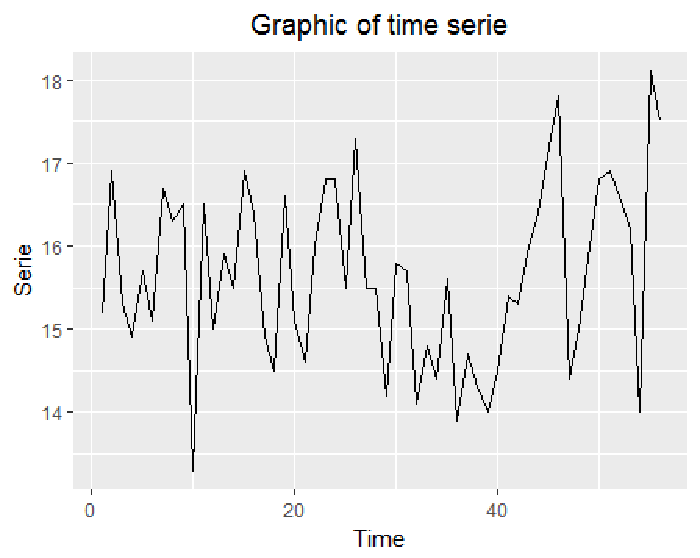
\includegraphics[width=0.7\columnwidth]{Rplot}
 \caption{Gráfico de uma série temporal de produção anual de cevada por acre.} \end{figure}


\begin{figure}[!hbt]
	\centering
	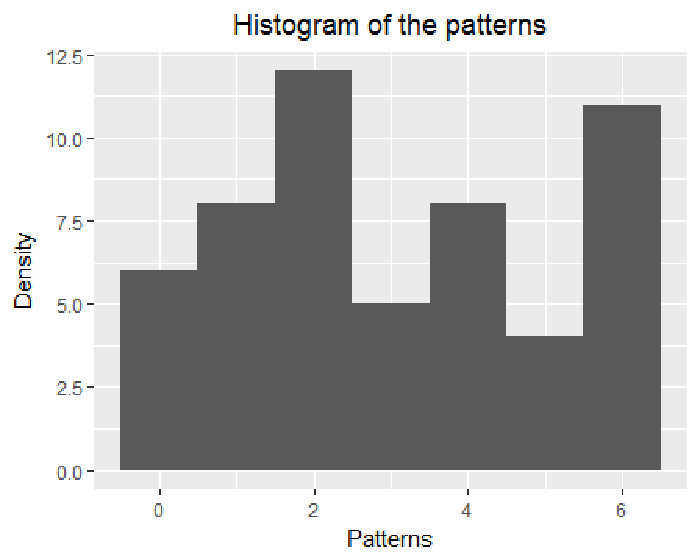
\includegraphics[width=0.7\columnwidth]{Rplot02}        
     \caption{Histograma de densidade dos padrões formados na série.}
\end{figure}


\begin{figure}[!hbt]
	\centering
	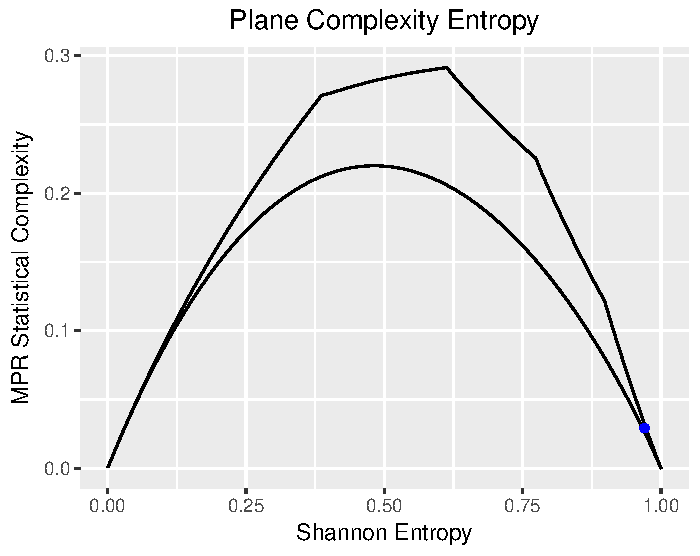
\includegraphics[width=0.7\columnwidth]{Rplot3}        
     \caption{Representação da série no plano Complexidade Entropia.}
\end{figure}


\begin{figure}[!hbt]
	\centering
	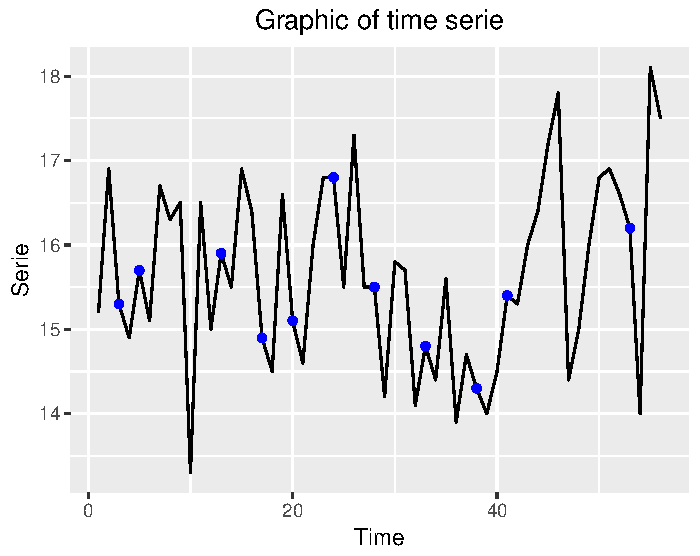
\includegraphics[width=0.7\columnwidth]{Rplot04}        
     \caption{Ilustração da representação na série dos pontos iniciais correspondentes ao padrão $\pi = (2,1,3)$ }
\end{figure}


\bibliographystyle{unsrt}
\bibliography{ref}

\end{document}